\section{Boundedness of hunger}\label{section: boundedness hunger}
The following lemmas will be useful in our discussion of the hunger game.
The first lemma shows that on a countable Markov chain, 
hunger stays uniformly bounded from below under the hunger game process,
including the removal and reinsertion of the chip 
if it reaches an absorbing state.

\begin{lemma}\label{lemma: hunger bounded lower}
Suppose we play the hunger game for a countable Markov chain, 
with an initial hunger vector $\mathbf{h}^{(0)}$ that is bounded below by $h_{min}\in\R$,
meaning $\h_i^{(0)} \geq h_{min}$ for all $i$.
Then hunger remains uniformly bounded below by $h_{min}-1$
under iteration of the hunger game process.
That is, suppose we have a sequence of hunger states 
$\mathbf{h}^{(1)}, \mathbf{h}^{(2)},\dots$ such that 
for each $k \geq 1$, $\mathbf{h}^{(k)}$ is reached 
from $\h^{(k-1)}$ by either firing the chip if it is not at an absorbing state
or removing and reinserting the chip if it is.
Then $\mathbf{h}^{(k)}_i \geq h_{min}-1$ holds for all $i$ and $k$.
\end{lemma}
\begin{proof}
Without loss of generality, we may take $h_{min}$ to be 0,
so that $\mathbf{h}_i^{(0)} \geq 0$ for all $i$.
Suppose our claim is false,
and let $k$ be the smallest index for which the claim fails,
so that $\h^{(k)}_i < -1$ for some $i$.
Consider the set $S$ of states whose hunger changed 
during the hunger game process from $\h^{(0)}$ to $\h^{(k)}$; 
this set must be finite, for each of the $k$ steps can only
change the hunger of finitely many states, and must contain $i$.
The total hunger of this set must be constant during this hunger game process
if we combine the process of removing a chip and inserting the next chip
into a single operation.
Let $h$ be the total hunger of $S$ throughout the process.
As the hunger of all states was originally bounded below by $0$,
we have $h \geq 0$.
Since in going from $\h^{(k-1)}$ to $\h^{(k)}$ we fired the chip to $i$,
$v_i$ must have been one of the hungriest vertices.
But in $\h^{(k-1)}$, $v_i$ must have had hunger $< 0$
(otherwise it could not have reached hunger $< -1$ in a single firing).
Since the hungers of the vertices in $S$ have nonnegative sum,
at least one of them must be nonnegative,
and hence $v_i$ could not have been one of the hungriest vertices.
This contradiction shows that hunger is bounded from below,
and more specifically that $h_{min}-1$ is a lower bound.
\end{proof}

The lemma remains true if one replaces $\geq$ by $>$
in both the hypothesis and the conclusion.

\bigskip

\cref{lemma: hunger bounded lower} only provides a uniform lower bound on hunger; a uniform upper bound on hunger does not exist in general for countable Markov chains.
One may construct Markov chains where depending on the location 
of chip insertion, hunger 
can grow arbitrarily large at a certain state.
As a specific example, 
consider the countably infinite Markov chain 
shown in \cref{fig:rem unbounded hunger harmonic}\,.
We have states $v_{i,j}$ for all integers $i \geq j \geq 0$, 
where $v_{0,0}$ is an absorbing state.
A walker at vertex $v_{i,j}$ for $i > j$ moves with equal probability 
to any vertex $v_{i,k}$ with $k>j$, 
in other words with probability $\frac{1}{i-j}$ to $v_{i,k}$ 
for all $j+1 \leq k \leq i$, 
and a walker at $v_{i,i}$ moves with probability 1 
to the absorbing vertex $v_{0,0}$.
Starting with $\mathbf{h}=\mathbf{0}$, 
inserting a chip at $v_{n,0}$ for $n>0$ 
causes the chip to move from $v_{n,0}$ to $v_{n,n}$, 
increasing the second coordinate by 1 each step 
(i.e. moving one position to the right at each step).
When the chip fires to $v_{n,n-1}$, 
state $v_{n,n}$ has hunger $1+\frac{1}{2}+\frac{1}{3}+\cdots+\frac{1}{n}$, 
the $n$th partial sum of the harmonic series. 
As the harmonic series diverges, by picking sufficiently large $n$, 
hunger can become arbitrarily large at $v_{n,n}$, 
and is thus not uniformly bounded under the hunger game process,
when chip removal and insertion are allowed.
\begin{figure}[htbp!]
    \centering
    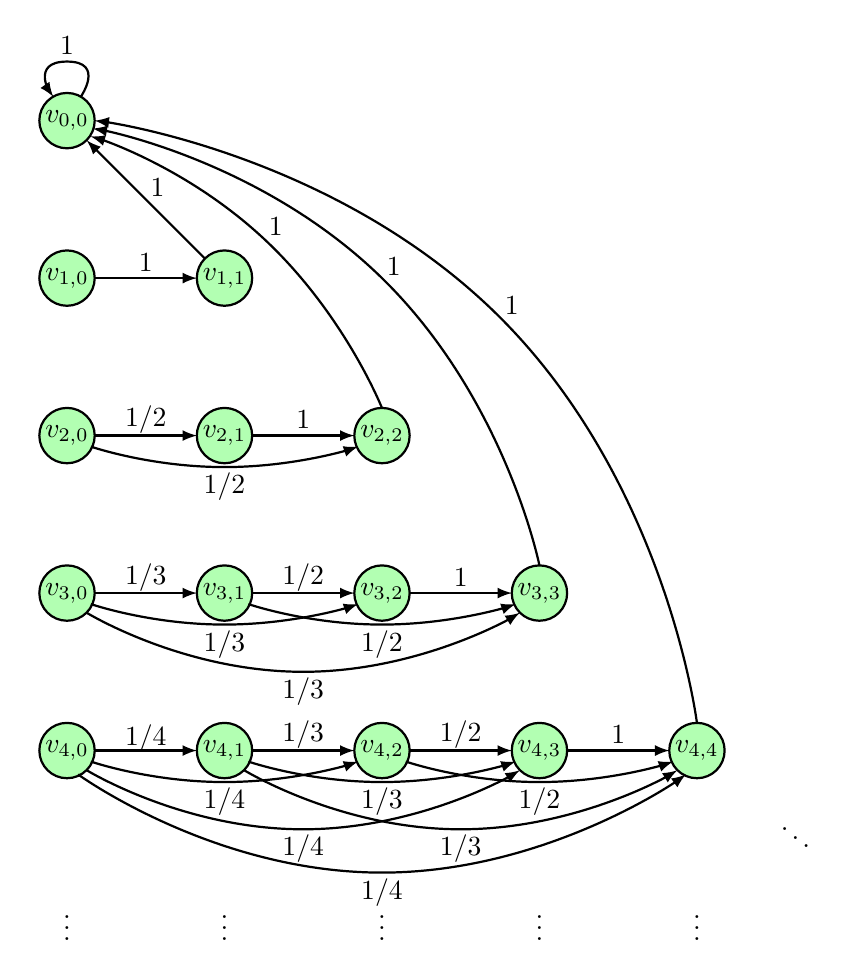
\begin{tikzpicture}[scale=0.5,font=\normalsize,baseline,thick]
        \filldraw[color=black,fill=green!30,thick] (0,0) circle (20pt);
        \node at (0,0) {$v_{0,0}$};
        \foreach \y in {1,...,4} {
        \foreach \x in {0,...,\y} {
            \filldraw[color=black,fill=green!30,thick] (4*\x, -4 * \y) circle (20pt);
            \node at (4*\x,-4 * \y) {$v_{\y,\x}$};
        }
        }
        \foreach \x in {0,...,4} {
            \node at (4*\x, -4*5-0.3) {$\vdots$};
        }
        \node at (4*4+2.5,-4*5+2) {$\ddots$};
        % Self-loop absorbing v_0
        \draw [->,>=latex] plot [smooth,tension=5] coordinates {(0+0.5*0.7,0.866*0.7) (0+0,1.5) (0-0.5*0.7,0.866*0.7)};
        \node at (0,1.9) {1};
        % Redirect to v_0
        \draw[->,>=latex] (4-0.5,-4+0.5) -- (0+0.5,0-0.5);
        \node at (2+0.3,-2+0.3) {1};
        \draw[->,>=latex] plot [smooth,tension=1] coordinates {(8,-8+0.7) (4+1,-4+1) (0+0.6,0-0.4)};
        \node at (4+1.3,-4+1.3) {1};
        \draw[->,>=latex] plot [smooth,tension=1] coordinates {(12,-12+0.7) (6+2,-6+2) (0+0.65,0-0.2)};
        \node at (6+2.3,-6+2.3) {1};
        \draw[->,>=latex] plot [smooth,tension=1] coordinates {(16,-16+0.7) (8+3,-8+3) (0+0.7,0-0)};
        \node at (8+3.3,-8+3.3) {1};
        % Edge weight 1
        \foreach \y in {1,...,4} {
            \draw[->,>=latex] (4*\y - 4+0.7, -4*\y) -- (4*\y -0.7, -4*\y);
            \node at (4*\y - 2,-4*\y + 0.4) {1};
        }
        % Edge weight 1/2
        \foreach \y in {2,...,4} {
            \draw[->,>=latex] (4*\y - 4*2 +0.7, -4*\y) -- (4*\y -4*1 -0.7, -4*\y);
            \node at (4*\y - 4*1 - 2, -4*\y + 0.4) {1/2};
            \draw [->,>=latex] plot [smooth,tension=1] coordinates {(4*\y-4*2+0.866*0.7,-4*\y - 0.4*0.7) (4*\y-4*1,-4*\y-0.8) (4*\y-0.866*0.7,-4*\y - 0.4*0.7)};
            \node at (4*\y-4*1,-4*\y-1.3) {1/2};
        }
        % Edge weight 1/3
        \foreach \y in {3,...,4} {
            \draw[->,>=latex] (4*\y - 4*3 +0.7, -4*\y) -- (4*\y -4*2 -0.7, -4*\y);
            \node at (4*\y - 4*2 - 2, -4*\y + 0.4) {1/3};
            \draw[->,>=latex] plot [smooth,tension=1] coordinates {(4*\y-4*3+0.866*0.7,-4*\y - 0.4*0.7) (4*\y-4*2,-4*\y-0.8) (4*\y-4*1-0.866*0.7,-4*\y - 0.4*0.7)};
            \node at (4*\y-4*2,-4*\y-1.3) {1/3};
            \draw[->,>=latex] plot [smooth,tension=1] coordinates {(4*\y-4*3+0.5,-4*\y-0.5) (4*\y-2*3,-4*\y - 2) (4*\y-0.5,-4*\y-0.5)};
            \node at (4*\y-2*3,-4*\y - 2 - 0.5) {1/3};
        }
        % Edge weight 1/4
        \foreach \y in {4,...,4} {
            \draw[->,>=latex] (4*\y - 4*4 +0.7, -4*\y) -- (4*\y -4*3 -0.7, -4*\y);
            \node at (4*\y - 4*3 - 2, -4*\y + 0.3) {1/4};
            \draw[->,>=latex] plot [smooth,tension=1] coordinates {(4*\y-4*4+0.866*0.7,-4*\y - 0.4*0.7) (4*\y-4*3,-4*\y-0.8) (4*\y-4*2-0.866*0.7,-4*\y - 0.4*0.7)};
            \node at (4*\y-4*3,-4*\y-1.3) {1/4};
            \draw[->,>=latex] plot [smooth,tension=1] coordinates {(4*\y-4*4+0.5,-4*\y-0.5) (4*\y-4*2.5,-4*\y - 2) (4*\y-4-0.5,-4*\y-0.5)};
            \node at (4*\y-2*5,-4*\y - 2 - 0.5) {1/4};
            \draw[->,>=latex] plot [smooth,tension=1] coordinates {(4*\y-4*4+0.4*0.7,-4*\y-0.866*0.7) (4*\y-4*2,-4*\y-3.1) (4*\y-4*0-0.4*0.7,-4*\y-0.866*0.7)};
            \node at (4*\y-4*2,-4*\y-3.6) {1/4};
        }
        
    \end{tikzpicture}
    \caption{A countably infinite absorbing Markov chain where hunger is not uniformly bounded under chip addition operators.}
    \label{fig:rem unbounded hunger harmonic}
\end{figure}

This example used a countably infinite state space, which is necessary for this unbounded behavior to occur.
As shown in the following lemma, for a finite Markov chain, 
hunger stays uniformly bounded from both sides under the hunger game process,
including the removal and reinsertion of the chip 
if it reaches an absorbing state.

\begin{lemma}\label{lemma: hunger bounded}
For a given hunger state $\h^{(0)}$ on a finite Markov chain, 
hunger remains uniformly bounded under the hunger game process.
In other words, there exist $a,b \in \R$ such that for any sequence
of hunger states $\h^{(1)},\h^{(2)},\dots$, where for each $k\geq 1$,
$\h^{(k)}$ is reached from $\h^{(k-1)}$ by either
firing the chip if it is not at an absorbing state
or removing and reinserting the chip if it is,
the inequality $a \leq \h^{(k)}_i \leq b$ holds for all $i$ and $k$.
\end{lemma}
\begin{proof}
The existence of a lower bound $a$ follows directly 
from \cref{lemma: hunger bounded lower}\,, 
as any hunger state on a finite Markov chain must be bounded.

As hunger is bounded from below by $a$ 
and total hunger $h$ is constant during the hunger game process, 
when we conceive of removing a chip and inserting the next chip 
as occurring simultaneously, 
the hunger of any single vertex cannot exceed $h-(n-1)a$, 
and thus hunger is bounded from above and $b$ exists.
\end{proof}

\begin{remark}\label{remark: finite orbit}
When all transition probabilities are rational
and the Markov chain has no absorbing states,
so that we never remove and reinsert the chip---which
introduces choice into the hunger game---we claim \cref{lemma: hunger bounded}
implies that the hunger game is eventually periodic.
Let $d$ be the least common multiple
of the denominators of all the transition probabilities.
% For any $\h^{(0)}$ there are only finitely many integer vectors $\v$ 
% such that the hunger vector $\h^{(0)} + H \v$ 
% satisfies the bounds of the Lemma
% (this follows from the fact that $H$ has corank 1).
For any $\h^{(0)}$, as each entry is uniformly bounded and may only
change by a multiple of $\frac{1}{d}$, there are only finitely
many values that $\h^{(k)}$ may take on as $k$ varies.
This implies that eventually we must have $\h^{(j)} = \h^{(i)}$ with $j > i$,
so that the hunger game has become periodic with period dividing $j-i$.
If we define $\v$ as the vector that counts
the number of visits to each state of the chain from time $i+1$ to time $j$,
we have $\v H = {\bf 0}$, implying that $\v$ is a stationary vector
and that $\frac{1}{j-i}\v$ is the stationary probability measure for the Markov chain.
Theorem \ref{theorem: irreducible fidelity converge stationary}
extends this claim, in a suitable asymptotic sense,
to situations in which the transition probabilities
are not all rational.
\end{remark}
